\documentclass[10pt,a4paper]{article}
\usepackage[latin1]{inputenc}
\usepackage{amsmath}
\usepackage{amsfonts}
\usepackage{amssymb}
\usepackage{fullpage}
\usepackage{graphicx}

\begin{document}
\title{J.D. Jackson Problem 9.11}
\author{Josh Orndorff \\ admin@joshorndorff.com}
\maketitle

\begin{figure}
\includegraphics[scale=.5]{Jackson9-11.png}
\end{figure}
We'll start by writing the charge density.  We could write it directly in spherical coordinates, but for clarity, we'll begin in the more intuitive Cartesian coordinates.
\begin{equation}
\rho=q\delta(x)\delta(y)[2\delta(z)-\delta(z-a\cos\omega t)-\delta(z+a\cos\omega t)]
\end{equation}

Now we can convert to spherical coordinates using the various delta function identities. Many useful delta identities can be found at wolfram math world.

\begin{equation}
\rho=\frac{q\delta(\theta)\delta(\phi)}{r^2 \sin\theta}[2\delta(r)-\delta(r-a\cos\omega t)-\delta(r+a\cos\omega t)]
\end{equation}

The problem specifies that $ka\ll 1$ so we can use equation 9.170 from the text to calculate the various $Q_{lm}$ terms.
\begin{equation}
Q_{lm}=\int r^l Y*_{lm}\rho \,\mathrm{d}V
\end{equation}

Directly substituting the forms of $Y*_{lm}$ and $\rho$ we get the following (where empty brackets indicate the bracked $r$-based delta functions from $\rho$).
\begin{equation}
Q_{lm}=\iiint r^l\sqrt{\frac{2l+1}{4\pi}\frac{(l-m)!}{(l+m)!}}P_{lm}(\cos\theta)e^{-im\phi}\frac{q\delta(\theta)\delta(\phi)}{r^2\sin\theta}[\cdots]r^2\sin\theta\,\mathrm{d}r\,\mathrm{d}\theta\,\mathrm{d}\phi
\end{equation}

Our charge distribution is azimuthally symetric, so all of the $m\neq0$ terms will be zero.  Looking only at the $m=0$ terms, the form simplifies nicely.
\begin{equation}
Q_{l0}=\iiint r^l\sqrt{\frac{2l+1}{4\pi}}P_l(\cos\theta)q\delta(\theta)\delta(\phi)[\cdots]\,\mathrm{d}r\,\mathrm{d}\theta\,\mathrm{d}\phi
\end{equation}

The $\theta$ and $\phi$ integrals are fairly easy to evaluate because of the delta functions.
\begin{equation}
Q_{l0}=q\sqrt{\frac{2l+1}{4\pi}}\left[
2\int_0^\infty r^l \delta(r) \,\mathrm{d}r
-\int_0^\infty r^l \delta(r-a\cos\omega t) \,\mathrm{d}r
-\int_0^\infty r^l \delta(r+a\cos\omega t) \,\mathrm{d}r
\right]
\end{equation}

Evaluating the integrals in the previous expression must be done carefully as the results will vary depending on the value of $l$.  For the $l=0$ case the first integral will cancel the second and third.  For all other $l$ the first integral is zero.  For odd $l$ the second and third integrals cancel each other, and for even $l$ the second and third terms add together.

So, for the non trivial values of $l$ we see that.
\begin{equation}
Q_{l0}=-2q\sqrt{\frac{2l+1}{4\pi}}a^l\cos^l \omega t
\end{equation}

The lowest non-trivial $Q$ is
\begin{equation}
Q_{20}=-\sqrt{\frac{5}{\pi}}qa^2\cos^2\omega t
\end{equation}

Using a trig identity, we can rewrite this in another form which emphasizes the fact that the oscilation frequency is actually $2\omega$.
\begin{equation}
Q_{20}=-\sqrt{\frac{5}{\pi}}qa^2\frac{1+\cos(2\omega t)}{2}
\end{equation}

To find the power per solid angle we can use equation 9.151.
\begin{equation}
\frac{\mathrm{d}P}{\mathrm{d}\Omega}=\frac{Z_0}{2k^2}\left|a(l,m)\right|^2\left|\mathbf{X}_{lm}\right|^2
\end{equation}

The table on page 437 give us
\begin{equation}
\left|\mathbf{X}_{20}\right|^2=\frac{15}{8\pi}\sin^2\theta\cos^2\theta
\end{equation}

Finding the $a_E(l,m)$ is not at all obvious.  I don't even know if it is supposed to depend on time or not.  But I do know the following from equation 9.169.
\begin{equation}
a(l,m)\approx \frac{ck^{l+2}}{i(2l+1)!!}\sqrt\frac{l+1}{l}Q_{lm}
\end{equation}

Alright, I'm not going to waste either of our time pretending I know what to do here.

\end{document}